\documentclass[a4paper,10pt]{article}
\usepackage{listings}
\usepackage{color}
\usepackage{algorithm2e}
\usepackage{graphicx}
\usepackage{epstopdf}
 
\definecolor{dkgreen}{rgb}{0,0.6,0}
\definecolor{gray}{rgb}{0.5,0.5,0.5}
\definecolor{mauve}{rgb}{0.58,0,0.82}
 
\lstset{ %
  language=C++,                % the language of the code
  basicstyle=\footnotesize,           % the size of the fonts that are used for the code
  numbers=left,                   % where to put the line-numbers
  numberstyle=\tiny\color{gray},  % the style that is used for the line-numbers
  stepnumber=1,                   % the step between two line-numbers. If it's 1, each line 
                                  % will be numbered
  numbersep=5pt,                  % how far the line-numbers are from the code
  backgroundcolor=\color{white},      % choose the background color. You must add \usepackage{color}
  showspaces=false,               % show spaces adding particular underscores
  showstringspaces=false,         % underline spaces within strings
  showtabs=false,                 % show tabs within strings adding particular underscores
  frame=single,                   % adds a frame around the code
  rulecolor=\color{black},        % if not set, the frame-color may be changed on line-breaks within not-black text (e.g. commens (green here))
  tabsize=2,                      % sets default tabsize to 2 spaces
  captionpos=b,                   % sets the caption-position to bottom
  breaklines=true,                % sets automatic line breaking
  breakatwhitespace=false,        % sets if automatic breaks should only happen at whitespace
  title=\lstname,                   % show the filename of files included with \lstinputlisting;
                                  % also try caption instead of title
  keywordstyle=\color{blue},          % keyword style
  commentstyle=\color{dkgreen},       % comment style
  stringstyle=\color{mauve},         % string literal style
  escapeinside={\%*}{*)},            % if you want to add LaTeX within your code
  morekeywords={*,...}               % if you want to add more keywords to the set
}

% Title Page
\title{Assignment 1: Introduction to Systems Programming}
\author{Francis Vo}


\begin{document}
	\maketitle

	\section{Mathematical Analysis}
		\subsection{Algorithm 1}
			\begin{algorithm}[H]
				\SetLine
				\linesnumbered
				\dontprintsemicolon
				\KwData{Integer array A of size N}
				\KwResult{Greatest Sum of Subarray}
				\For{$i \gets 0$ \KwTo $N$}{
					\For{$j \gets i$ \KwTo $N$}{
						$s \gets 0$\;
						\For{$k \gets i$ \KwTo $j$}{
							$s \gets s + A[k]$\;
						}
						\If{$s > max$}{
							 $max \gets s$\;
						}
					}
				}
			\caption{Pseudocode for Basic Enumeration}
			\end{algorithm}
		\subsection{Algorithm 2}
			\begin{algorithm}[H]
				\SetLine
				\linesnumbered
				\dontprintsemicolon
				\KwData{Integer array A of size N}
				\KwResult{Greatest Sum of Subarray}
				\For{$i \gets 0$ \KwTo $N$}{
					$s \gets 0$\;
					\For{$j \gets i$ \KwTo $N$}{
						 $s \gets A[j]$\;
						 \If{$s > max$}{
							 $max \gets s$\;
						 }
					}
				}
			\caption{Pseudocode for Better Enumeration}
			\end{algorithm}
		\subsection{Algorithm 3}
			\begin{algorithm}[H]
				\SetLine
				\linesnumbered
				\dontprintsemicolon
				\KwData{Integer array A of size N}
				\KwResult{Greatest Sum of Subarray}
% 				\Function{MaxSubarray}{$A$}{
% 					
% 				}
% 				\Function{MaxSubarray_recursion}{$A$}
% 					\If{A.size() <= 1}{
% 						\Return SUM = A[0], SUM_LEFT = A[0], SUM_RIGHT = A[0], MAX = A[0]
% 					}
% 					Left_results = MaxSubarray_recursion(A.Left_Side)
% 					Right_results = MaxSubarray_recursion(A.Right_Side)
% 					
% 				\EndFunction
			\caption{Pseudocode for Divide and Conquer}
			\end{algorithm}

	\section{Theoretical Correctness}

	\section{Testing}
	931678074 - 5703
	\newline
	930569466 - 8184
	\newline
	932086449 - 4949 
\newpage
	\section{Experimental Analysis}
		\subsection{Algorithm 1}
		
\begin{figure}[!htb]
\centering
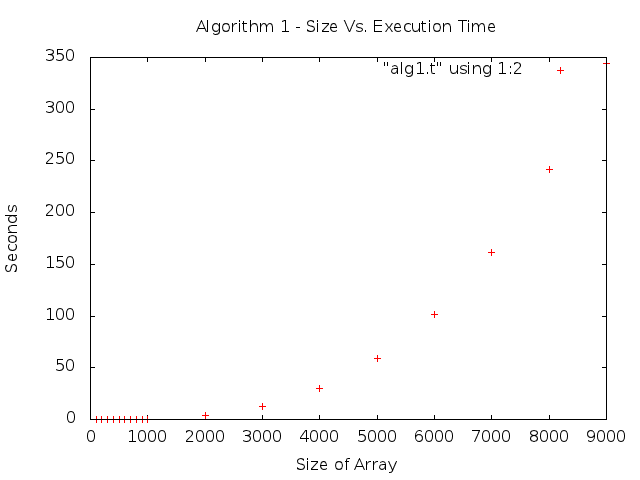
\includegraphics[scale=.5]{timingfiles/alg1plot.png}
\end{figure}
\begin{figure}[!htb]
\centering
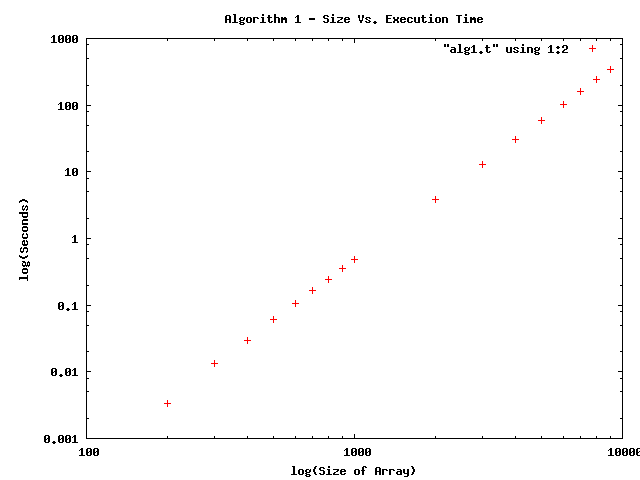
\includegraphics[scale=.5]{timingfiles/alg1plotlog.png}
\end{figure}
		\newpage
		\subsection{Algorithm 2}
\begin{figure}[!htb]
\centering
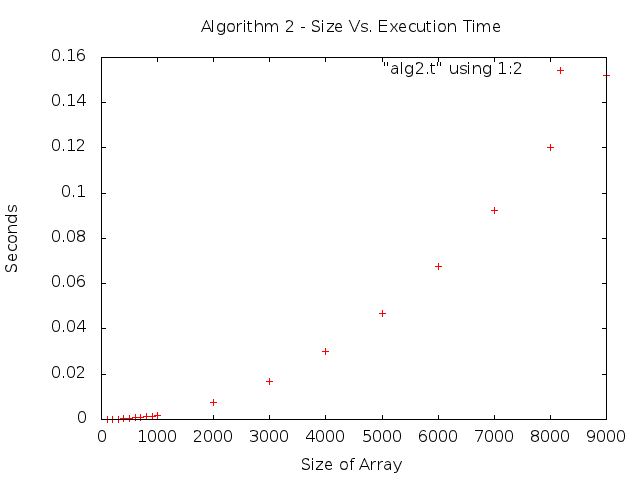
\includegraphics[scale=.5]{timingfiles/alg2plot.png}
\end{figure}
\begin{figure}[!htb]
\centering
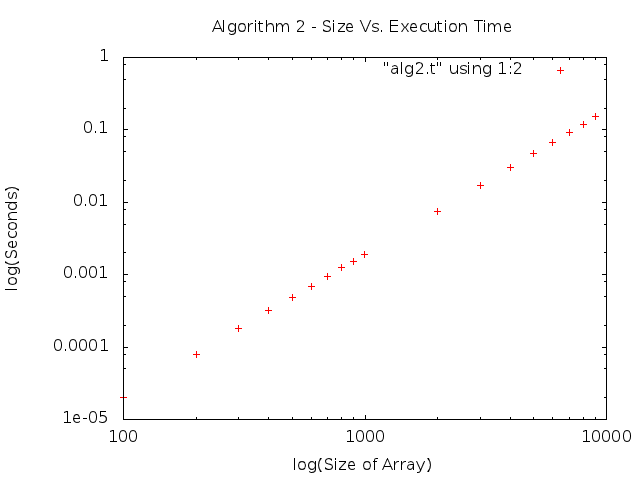
\includegraphics[scale=.5]{timingfiles/alg2plotlog.png}
\end{figure}
		\newpage
		\subsection{Algorithm 3}
\begin{figure}[!htb]
\centering
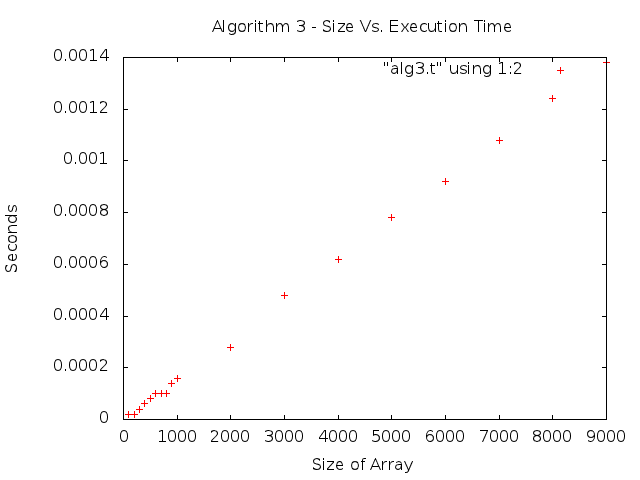
\includegraphics[scale=.5]{timingfiles/alg3plot.png}
\end{figure}
\begin{figure}[!htb]
\centering
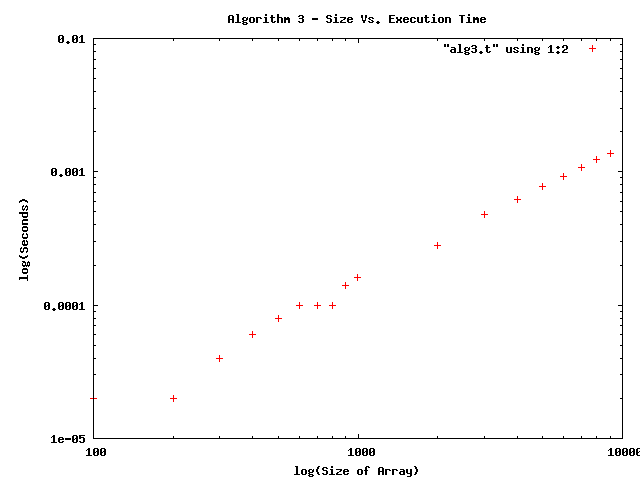
\includegraphics[scale=.5]{timingfiles/alg3plotlog.png}
\end{figure}
\newpage

	\section{Extrapolation and Interpretation}
		\subsection{Extrapolation}
			
		\subsection{Interpretation}
		\subsection{Algorithm 1}
			\subsubsection{Extrapolation}
				$f(n) = 4.71599 \times 10^{-10} \times n^3$\\
				$f(n) = 3600 \to n = 19690$\\
			\subsubsection{Interpretation}
				Slope $= 2.99734$
		
		\subsection{Algorithm 2}
			\subsubsection{Extrapolation}
				$f(n) = 1.87761 \times 10^{-9} \times n^2$\\
				$f(n) = 3600 \to n = 1384678$
			\subsubsection{Interpretation}
				Slope $= 1.99602$
		\subsection{Algorithm 3}
			\subsubsection{Extrapolation}
				$f(n) = 1.74832 \times 10^{-8} \times n \times log(n)$\\
				$f(n) = 3600 \to n = 8984428998 =8.98 \times 10^9$
			\subsubsection{Interpretation}
				Slope $= 1.00506$

	\newpage
	\section{Code}
		\subsection{Algorithm 1}
		\lstinputlisting[language=C++]{alg1.cpp}
		\newpage
		\subsection{Algorithm 2}
		\lstinputlisting[language=C++]{alg2.cpp}
		\newpage
		\subsection{Algorithm 3}
		\lstinputlisting[language=C++]{alg3.cpp}
		

\end{document}
